\documentclass{article}

\usepackage{url}
\usepackage{fancyhdr}
\usepackage{extramarks}

\usepackage{amsmath}
\usepackage{amsthm}
\usepackage{amsfonts}
\usepackage{tikz}
\usetikzlibrary{3d}
\usepackage[plain]{algorithm}
\usepackage{algpseudocode}
\usepackage{braket}
\usepackage{enumerate}
\usepackage{paralist}
\usepackage{listings}


%
% Basic Document Settings
%

\topmargin=-0.45in
\evensidemargin=0in
\oddsidemargin=0in
\textwidth=6.5in
\textheight=9.0in
\headsep=0.25in

\linespread{1.1}

\pagestyle{fancy}
\lhead{Habib University}
\chead{\hmwkClass, \hmwkTitle}
\rhead{\firstxmark}
\lfoot{\lastxmark}
\cfoot{\thepage}

\renewcommand\headrulewidth{0.4pt}
\renewcommand\footrulewidth{0.4pt}

\setlength\parindent{0pt}

\definecolor{mGreen}{rgb}{0,0.6,0}
\definecolor{mGray}{rgb}{0.5,0.5,0.5}
\definecolor{mPurple}{rgb}{0.58,0,0.82}
\definecolor{backgroundColour}{rgb}{0.95,0.95,0.92}

\lstdefinestyle{CStyle}{
    backgroundcolor=\color{backgroundColour},
    commentstyle=\color{mGreen},
    keywordstyle=\color{magenta},
    numberstyle=\tiny\color{mGray},
    stringstyle=\color{mPurple},
    basicstyle=\footnotesize,
    breakatwhitespace=false,
    breaklines=true,
    captionpos=b,
    keepspaces=true,
    numbers=left,
    numbersep=5pt,
    showspaces=false,
    showstringspaces=false,
    showtabs=false,
    tabsize=2,
    language=C
}

%
% Create Problem Sections
%


\newcommand{\enterProblemHeader}[1]{
	\nobreak\extramarks{}{Problem \arabic{#1} continued on next page\ldots}\nobreak{}
	\nobreak\extramarks{Problem \arabic{#1} (continued)}{Problem \arabic{#1} continued on next page\ldots}\nobreak{}
}

\newcommand{\exitProblemHeader}[1]{
	\nobreak\extramarks{Problem \arabic{#1} (continued)}{Problem \arabic{#1} continued on next page\ldots}\nobreak{}
	\stepcounter{#1}
	\nobreak\extramarks{Problem \arabic{#1}}{}\nobreak{}
}

\setcounter{secnumdepth}{0}
\newcounter{partCounter}
\newcounter{homeworkProblemCounter}
\setcounter{homeworkProblemCounter}{1}
\nobreak\extramarks{Problem \arabic{homeworkProblemCounter}}{}\nobreak{}

%
% Homework Problem Environment
%
% This environment takes an optional argument. When given, it will adjust the
% problem counter. This is useful for when the problems given for your
% assignment aren't sequential. See the last 3 problems of this template for an
% example.
%
\newenvironment{homeworkProblem}[1][-1]{
	\ifnum#1>0
	\setcounter{homeworkProblemCounter}{#1}
	\fi
	\section{Problem \arabic{homeworkProblemCounter}}
	\setcounter{partCounter}{1}
	\enterProblemHeader{homeworkProblemCounter}
}{
	\exitProblemHeader{homeworkProblemCounter}
}

%
% Homework Details
%   - Title
%   - Due date
%   - Class
%   - Section/Time
%   - Instructor
%   - Author
%

\newcommand{\hmwkTitle}{Assignment\ \#3}
\newcommand{\hmwkDueDate}{March 30, 2024, 11.59pm}
\newcommand{\hmwkClass}{CS 201 - Data Structures II}
\newcommand{\hmwkClassInstructor}{Muhammad Mobeen Movania (L1),\\ Syeda Saleha Raza (L2),\\ Faisal Alvi (L3, L4),\\ Abdullah Zafar (L5).}
\newcommand{\hmwkAuthorName}{\textbf{Student 1 Name, ID} \and \textbf{Student 2 Name, ID}}

%
% Title Page
%

\title{
	\vspace{2in}
	\textmd{\textbf{\hmwkClass:\\ \hmwkTitle}}\\
	\normalsize\vspace{0.1in}\small{\hmwkClassInstructor}\\
	\normalsize\vspace{0.1in}\small{Due\ on\ \hmwkDueDate}\\
	\vspace{3in}
}

\author{\hmwkAuthorName}
\date{}

\renewcommand{\part}[1]{\textbf{\large Part \Alph{partCounter}}\stepcounter{partCounter}\\}

%
% Various Helper Commands
%

% Useful for algorithms
\newcommand{\alg}[1]{\textsc{\bfseries \footnotesize #1}}

% For derivatives
\newcommand{\deriv}[1]{\frac{\mathrm{d}}{\mathrm{d}x} (#1)}

% For partial derivatives
\newcommand{\pderiv}[2]{\frac{\partial}{\partial #1} (#2)}

% Integral dx
\newcommand{\dx}{\mathrm{d}x}

% Alias for the Solution section header
\newcommand{\solution}{\textbf{\large Solution}}

% Probability commands: Expectation, Variance, Covariance, Bias
\newcommand{\E}{\mathrm{E}}
\newcommand{\Var}{\mathrm{Var}}
\newcommand{\Cov}{\mathrm{Cov}}
\newcommand{\Bias}{\mathrm{Bias}}

\begin{document}
	
\maketitle
	
\pagebreak
\section{Instructions}
This assignment document consists of two problems.

\begin{itemize} 
	\item \underline{Problem 1} is a programming based question which requires implementation. It must be submitted by pushing all your code files to the Github repository. This problem is worth 40 points.
	\item \underline{Problem 2} is a theoretical question which requires analysis. It should be completed and submitted within this document as a pdf on Canvas. This problem is worth 20 points.
	

\end{itemize}

\newpage
\begin{homeworkProblem} (40 points) [\textbf{Implementing File System Index using AVL and BST}] 

You have learned about database indexes in CS 355 Database Systems. Indexes are used across various types of software, including the database management system (DBMS), operating system, and other applications to efficiently search and retrieve data. For example, an index in a database is a sorted list of key values with the storage locations of rows in the table that contain the key value. Similarly, the file system index in an operating system contains an entry for each file name and the starting location of the file on disk. Each key in the index is associated with a particular pointer (or a list of pointers) to a record in the data file, as shown in Figure \ref{fig1}.

\begin{figure}[htbp]
    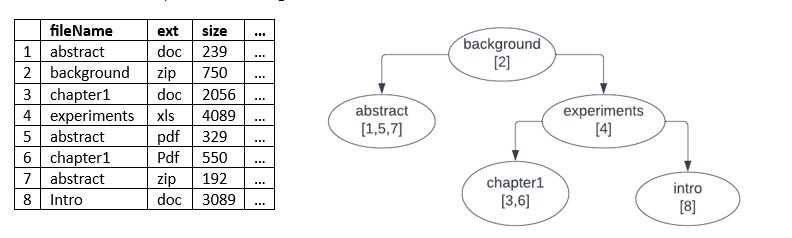
\includegraphics[width=\linewidth]{./fig/fig1.png}
    \caption{AVL index created on a list of files.}
    \label{fig1}
\end{figure}

Self-balancing trees have been a popular choice to store indexes. Most commercial DBMSs use B-Tree/B+ Tree to maintain indexes. In this question, you will build your own BST and AVL tree based indexes to index files stored on your file system. These indexes will help you building a mini file explorer that can efficiently search for files on different criteria. The question involves:

\begin{itemize}
\item	Loading file details (FileName, Size,accessedOn, modifiedOn,Type,path) from a given folder/CSV file on your file system
\item	Indexing these files using BST and AVL tree for efficient search
\item	Using these indexes in your mini file explorer to search for files on different criteria
\item	Performing a comparison of BST vs AVL indexes in terms of number of nodes that they traverse during different search operations. For this, we have used a dataset adapted from the Kaggle dataset on \url{https://www.kaggle.com/datasets/cogitoe/crab}.

\end{itemize}
This question provides you a minimal code structure and function interfaces that you have to maintain in your solution. Besides that, you are free to devise your own structure for the implementation of tree and its helper functions. 


\subsection{Dataset}

You have been given three datasets and their details are as follows:
\begin{enumerate}
\item Small dataset which contains 1,000 records and is represented by the \texttt{Small.csv} file.
\item Medium dataset which contains 10,000 records and is represented by the \texttt{Medium.csv} file.
\item Large dataset which contains 50,000 records and is represented by the \texttt{Large.csv} file.
\end{enumerate}

In addition, you have been given a sample dataset which contains 6 enteries for testing purposes.

% Please add the following required packages to your document preamble:
% \usepackage{graphicx}
\begin{table}[htbp]
\centering
\resizebox{\columnwidth}{!}{%
\begin{tabular}{|l|l|l|l|l|l|}
\hline
Filename & Type & Size  & accessedOn        & modifiedOn           & path                                            \\ \hline
15420-8  & zip  & 99661 & 2016-10-14T21:21:17 & 2005-03-21T12:35:18 & /gutenberg/www.gutenberg.lib.md.us/15420-8.zip  \\ \hline
15420-8  & zip  & 99761 & 2016-10-14T21:21:17 & 2005-03-25T12:35:18 & /gutenberg1/www.gutenberg.lib.md.us/15420-8.zip \\ \hline
15420-9  & zip  & 99631 & 2016-10-14T21:21:17 & 2005-03-22T12:35:18 & /gutenberg/www.gutenberg.lib.md.us/15420-9.zip  \\ \hline
15420-10 & zip  & 99561 & 2016-10-14T21:21:17 & 2005-03-23T12:35:18 & /gutenberg/www.gutenberg.lib.md.us/15420-10.zip \\ \hline
15420-11 & zip  & 99961 & 2016-10-14T21:21:17 & 2005-03-24T12:35:18 & /gutenberg/www.gutenberg.lib.md.us/15420-11.zip \\ \hline
15420-12 & zip  & 99861 & 2016-10-14T21:21:17 & 2005-03-25T12:35:18 & /gutenberg/www.gutenberg.lib.md.us/15420-12.zip \\ \hline

\end{tabular}%
}
\caption{Sample Dataset}
\end{table}


\subsection{Code Structure}
The code base contains four main classes and their description are as follows:
\begin{enumerate}
\item The \texttt{FileSystem} class provides the functionality of loading file system data from a CSV file, and then storing it into a vector so that it can be later used to create File System Index.

\item The \texttt{BSTIndex} class represents a binary search tree index structure designed to efficiently organize and search file system data. It utilizes a binary search tree composed of TreeNode structures, each containing a key for indexing purposes and a vector storing the indices of file system entries associated with that key. This class provides methods for creating the index, adding new entries, and searching a particular entry.

\item The \texttt{AVLIndex} class extends the functionality of {BSTIndex} to implement an AVL tree-based index structure, which automatically balances itself to maintain optimal performance during insertion operations. It inherits from BSTIndex and overrides the add  methods to incorporate AVL tree balancing logic. 

\item The \texttt{FileExplorer} class implements a File System Explorer. It maintains a index based on Filename and modifiedOn using either AVL or BST.  It provides methods for searching files by name, date, name and date combination, name and size combination, and files created during a specified date range.


\end{enumerate}


\subsection{Required Tasks}
\begin{itemize}
\item Implement BST and AVL trees to build and maintain indexes on given file data. The index will be created on a given key and each node of the index will store a list of file records having that key. To perform this task, you have to implement the following methods in the \texttt{BSTIndex} class: 
\begin{itemize}
\item	\texttt{void CreateIndex(vector<FileSystemEntry> \&Data, const string \&IndexType)} – will create index on the given key in files data
\item	\texttt{void Add(const int i, const string \&Key)} – will add a new key to the index along with the details of files containing that key.

\end{itemize}
\item
Searching works the same way in both BST and AVL tree. Implement the following generic method in the BSTIndex class.
\begin{itemize}
\item  \texttt{std::pair<std::vector<int>, int> Search(const string \&Key)} – traverses the index to return details of a given key. This method also returns number of nodes visited while searching for the given key.
\end{itemize}
\item 
Now you will use these indexes to build your mini file explorer. Your file explorer will use either BST/AVLIndex to perform searches on various criteria. The explorer will create index on \texttt{FileName} and \texttt{lastModifiedOn} and provides following options to search for files:
\begin{itemize}
\item \texttt{FileExplorer(const string \&type, const string \&csv\_file)} – the constructor that creates indexes of the given type on filename and lastModified date. 
\item	\texttt{void FindByName(const string \&filename, const string \&output\_path)}– Saves the file paths having the given name in a text file at the provided directory.
\item	\texttt{void FindByDate(const string \&date, const string \&output\_path)} - Saves the file paths that  were last modified on the given date in a text file at the provided directory
\item	\texttt{void FindByNameAndDate(const string \&filename, const string \&date, const string \&output\_path)}   - This method first queries over both indexes separately for the given name and date and then saves the intersection of their results in a text file at the provided directory. 
\item	\texttt{void FindByNameAndSize(const string \&filename, const int size, const string \&output\_path)}– This method first finds the files of the given name and then further filters them on size. The results are then saved in a text file at the provided directory.
\item	\texttt{void FindFilesCreatedDuring(const string \&date1, const string \&date2, const string \&output\_path)} – This method finds the files last modified during the given data range (inclusive) and saves the file paths in a text file at the provided directory. \\
\textbf{Note: AVL trees are not ideal for range-based queries. However, you have no other choice. Let’s not iterate over the whole tree and try to traverse as few nodes as possible to perform this task.}
\end{itemize}



\end{itemize}

\vspace{0.5cm}

\subsection{Testing}
You can test the correctness of your implementation by executing the provided \texttt{Pytest} file \texttt{test\_file\_explorer.py}. The Pytest file compares the output files, which are generated by your program and stored in the output folder, with the expected output files stored in the \texttt{test-output} folder. You can execute the \texttt{Pytest} file by typing the following command in the terminal:

\begin{lstlisting}[language=bash, caption={Executing Pytest file}, label={list1}, style=CStyle]
pytest test_file_explorer.py
\end{lstlisting}

\textbf{Note: For more guidance on how to execute Pytest files, please course staff during their office hours}

\subsection{Grading Criteria}
The rubric for this homework is as follows:
\begin{itemize}
\item 10 points (BST) (Correctness +  Implementation)
\item 15 points (AVL) (Correctness + Implementation)
\item 15 points (FileExplorer) (Correctness + Implementation)
\end{itemize}
 
Penalties
\begin{itemize}
\item (-5) Code compiles with warnings
\item (-5) OOP Inheritance not applied correctly between AVL and BST
\item (-5) Implementation does not match the provided function signature.
\item (-5) GitHub repository does not follow appropriate structure. All the code files should be in the code folder and output files in the output folder.
\end{itemize}

\vspace{0.5cm}

\textbf{Compilation Guidelines:} Before proceeding with submission, kindly verify that your code compiles utilizing the \textbf{C++17} standard.  


\end{homeworkProblem}
\bigskip

\newpage
\begin{homeworkProblem}

(20 points) [\textbf{Analysis}]Assume that your FileExplorer has maintained separate AVL tree-based indexes for C and D drives on your hard disk. Now you have decided to merge them and have a unified index for the whole file system. Rather than re-creating the index from scratch, you want to combine existing indexes in an efficient way. Write pseudocode to combine two indexes with the complexity of $O (m + n)$. where $m$ and $n$ are number of nodes in two indexes.



\end{homeworkProblem}



\vspace{0.5cm}

Due date: March 30, 2024, 11:59 PM



\end{document}

